% generated by scripts/pkl_to_latex.py
% source PKL : thermal_v1_L6_Ne6_U10_t1_mode-uniform_tpall_t2all_tperpall_nmin2_solver-gcg_restarts2_iter200_kmax4_tol1em09_cut10_adaptive1_step5_clusteravg1_T0to1_N40-98c4f0fd07f2_knone_diag0.pkl
% scan type  : Tscan
% state      : gs
% x-max cap  : 0.5
% requires   : \usepackage{pgfplots} \pgfplotsset{compat=1.18}
% colours match the matplotlib PDF (tab10 cycle)
\definecolor{gmeC0}{HTML}{1F77B4}
\definecolor{gmeC1}{HTML}{FF7F0E}
\definecolor{gmeC2}{HTML}{2CA02C}
\definecolor{gmeC3}{HTML}{D62728}
\definecolor{gmeC4}{HTML}{9467BD}
\definecolor{gmeC5}{HTML}{8C564B}
\definecolor{gmeC6}{HTML}{E377C2}
\definecolor{gmeC7}{HTML}{17BECF}

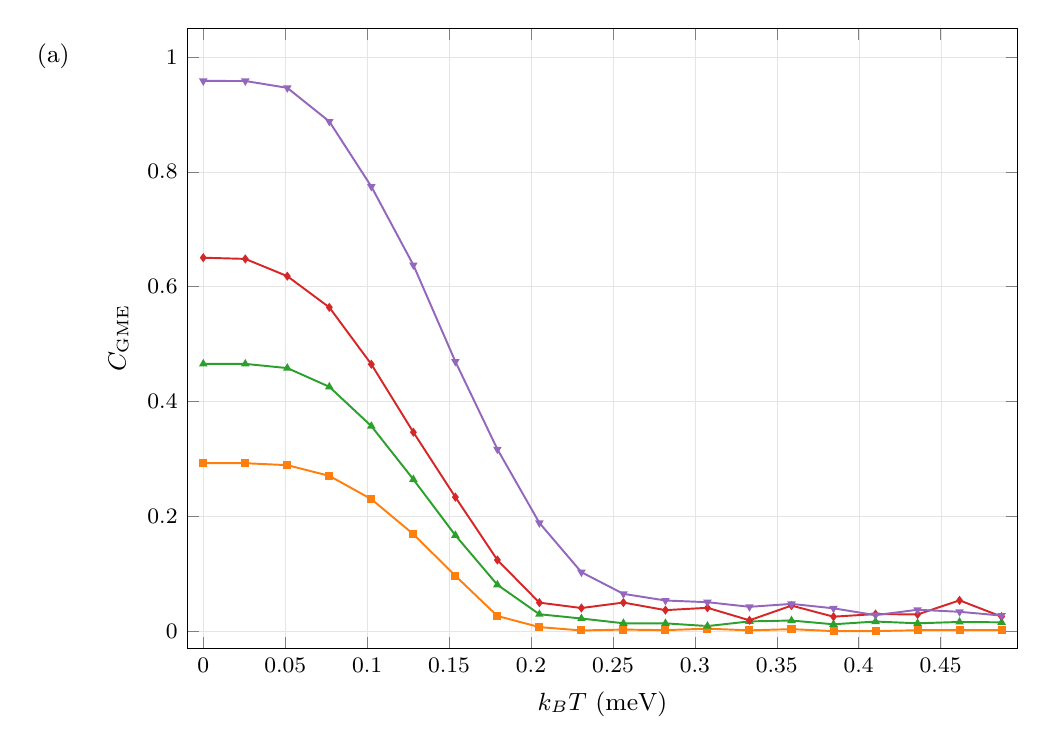
\begin{tikzpicture}
  \begin{axis}[
    width=\columnwidth,
    height=0.78\columnwidth,
    xlabel={$k_B T$ (meV)},
    ylabel={$C_{\mathrm{GME}}$},
    grid=both,
    grid style={line width=.1pt, draw=gray!20},
    tick label style={font=\footnotesize\rmfamily, /pgf/number format/fixed},
    label style={font=\small\rmfamily},
    scaled ticks=false,
    legend style={font=\scriptsize\rmfamily, draw=gray!40, at={(0.5,1.03)}, anchor=south, /tikz/every even column/.append style={column sep=6pt}},
    legend cell align={left},
    legend columns=2,
    ymin=-0.03,
    ymax=1.05,
    xmin=-0.00974359,
    xmax=0.496923,
    after end axis/.append code={\node[anchor=east, font=\small\rmfamily] at (axis description cs:-0.13,0.954) {(a)};},
  ]
    \addplot[color=gmeC1, mark=square*, mark size=1.1pt, line width=0.7pt] coordinates {
        (0,0.292503) (0.025641,0.292487) (0.051282,0.289105) (0.076923,0.270464)
        (0.102564,0.229909) (0.128205,0.168936) (0.153846,0.096415) (0.179487,0.026412)
        (0.205128,0.007085) (0.230769,0.001241) (0.25641,0.002766) (0.282051,0.001766)
        (0.307692,0.004402) (0.333333,0.001405) (0.358974,0.003529) (0.384615,0.000111)
        (0.410256,0.000106) (0.435897,0.001655) (0.461538,0.001806) (0.487179,0.001802)
    };
    \addplot[color=gmeC2, mark=triangle*, mark size=1.1pt, line width=0.7pt] coordinates {
        (0,0.465518) (0.025641,0.465429) (0.051282,0.458153) (0.076923,0.425559)
        (0.102564,0.357143) (0.128205,0.26434) (0.153846,0.166941) (0.179487,0.080776)
        (0.205128,0.029465) (0.230769,0.022053) (0.25641,0.013754) (0.282051,0.013619)
        (0.307692,0.008894) (0.333333,0.017021) (0.358974,0.018532) (0.384615,0.012011)
        (0.410256,0.016794) (0.435897,0.013699) (0.461538,0.016055) (0.487179,0.015403)
    };
    \addplot[color=gmeC3, mark=diamond*, mark size=1.1pt, line width=0.7pt] coordinates {
        (0,0.650363) (0.025641,0.648271) (0.051282,0.618207) (0.076923,0.563876)
        (0.102564,0.464795) (0.128205,0.346454) (0.153846,0.233467) (0.179487,0.123938)
        (0.205128,0.049676) (0.230769,0.040319) (0.25641,0.049833) (0.282051,0.036622)
        (0.307692,0.040715) (0.333333,0.018938) (0.358974,0.044547) (0.384615,0.025242)
        (0.410256,0.029762) (0.435897,0.029107) (0.461538,0.053662) (0.487179,0.025318)
    };
    \addplot[color=gmeC4, mark=triangle*, mark size=1.1pt, mark options={rotate=180}, line width=0.7pt] coordinates {
        (0,0.958182) (0.025641,0.958106) (0.051282,0.946136) (0.076923,0.887551)
        (0.102564,0.774311) (0.128205,0.637655) (0.153846,0.469511) (0.179487,0.316809)
        (0.205128,0.188538) (0.230769,0.102704) (0.25641,0.064995) (0.282051,0.053415)
        (0.307692,0.050481) (0.333333,0.04241) (0.358974,0.047484) (0.384615,0.039819)
        (0.410256,0.027898) (0.435897,0.037312) (0.461538,0.033734) (0.487179,0.027162)
    };
  \end{axis}
\end{tikzpicture}
